\documentclass[journal]{IEEEtran}

% *** CITATION PACKAGES ***
%
%\usepackage{cite}
\usepackage{capt-of}%%To get the caption
\usepackage{gensymb}
\usepackage{graphicx} %package to manage images
\graphicspath{ {./images/} }
\usepackage{wrapfig}

\usepackage[style=ieee]{biblatex}
\DeclareLanguageMapping{english}{english-apa}
\addbibresource{references.bib}
\usepackage[justification=centering]{caption}

\usepackage{setspace}

\usepackage{hhline}

\usepackage{booktabs}

% *** GRAPHICS RELATED PACKAGES ***
%
\ifCLASSINFOpdf
  % \usepackage[pdftex]{graphicx}
  % declare the path(s) where your graphic files are
  % \graphicspath{{../pdf/}{../jpeg/}}
  % and their extensions so you won't have to specify these with
  % every instance of \includegraphics
  % \DeclareGraphicsExtensions{.pdf,.jpeg,.png}
\else
  % or other class option (dvipsone, dvipdf, if not using dvips). graphicx
  % will default to the driver specified in the system graphics.cfg if no
  % driver is specified.
  % \usepackage[dvips]{graphicx}
  % declare the path(s) where your graphic files are
  % \graphicspath{{../eps/}}
  % and their extensions so you won't have to specify these with
  % every instance of \includegraphics
  % \DeclareGraphicsExtensions{.eps}
\fi
% graphicx was written by David Carlisle and Sebastian Rahtz. It is
% required if you want graphics, photos, etc. graphicx.sty is already
% installed on most LaTeX systems. The latest version and documentation
% can be obtained at: 
% http://www.ctan.org/pkg/graphicx
% Another good source of documentation is "Using Imported Graphics in
% LaTeX2e" by Keith Reckdahl which can be found at:
% http://www.ctan.org/pkg/epslatex
%
% latex, and pdflatex in dvi mode, support graphics in encapsulated
% postscript (.eps) format. pdflatex in pdf mode supports graphics
% in .pdf, .jpeg, .png and .mps (metapost) formats. Users should ensure
% that all non-photo figures use a vector format (.eps, .pdf, .mps) and
% not a bitmapped formats (.jpeg, .png). The IEEE frowns on bitmapped formats
% which can result in "jaggedy"/blurry rendering of lines and letters as
% well as large increases in file sizes.
%
% You can find documentation about the pdfTeX application at:
% http://www.tug.org/applications/pdftex

\begin{document}

\begin{titlepage}
    {\centering
        \vspace*{20em}
        {
        \huge 
        \begin{spacing}{1.5}
            Measuring the Internal Resistance of an \\
            Alkaline and Nickel Metal Hydride Battery

            
            \\
            \\
            \bigskip
            \large
            Circuits Fundamentals Lab 3, (ENGR-UH 2019-LAB)
        \end{spacing}

        }
        
    }
    \vfill
    
    {
    \large
    
    \begin{spacing}{1.5}
    \noindent Barkin Simsek, {\it {bs3528@nyu.edu}} 
    \\
    Nishant Aswani, {\it {nsa325@nyu.edu}}
    \\
    Table Number: \#Workstation 8% <-this % stops a space
    \end{spacing}
    }


\end{titlepage}
\pagenumbering{gobble}
\clearpage\mbox{}
\clearpage
\pagenumbering{arabic}
\setcounter{page}{1}

%\title{Demonstration of a Voltage Divider With A Variable Resistor}

%\author{Barkin Simsek,~\IEEEmembership{bs3528@nyu.edu};
%Nishant Aswani,~\IEEEmembership{nsa325@nyu.edu}
%\\ Table Number: \#}% <-this % stops a space


% The paper headers
\markboth{Simsek, Aswani, Circuits Fundamentals Lab 2019}%
{}

% make the title area
%\maketitle

% As a general rule, do not put math, special symbols or citations
% in the abstract or keywords.
\begin{abstract}
In this experiment, the internal resistance of two different kinds of batteries (Nickel metal-hydride and Alkaline) were calculated by connecting 3 different external loads (5 \ohm, 10 \ohm, 15 \ohm). The voltage drop across the resistors and the open circuit voltage of the battery were measured to calculate the internal resistance of the batteries. Finally, the collected data was fit into a curve and the power dissipated at the internal resistor and external load was compared.
\end{abstract}


%Percenta of power being consumed at the internal resistence

%What happens to voltage when external load is connected and current %consumption increaased

%Formula derivation
%Application 


\section{Introduction}
\IEEEPARstart{T}\lowercase{he} purpose of this exercise was to measure the internal resistance of a battery using a simple resistor circuit, compare the power absorbed between the internal resistor ($R_{in}$) and the resistor in the circuit ($R_{ex}$), and describe the relationship between the voltage drop and current load across $R_{ex}$. Comparing the power consumption of the internal resistor to that of the load resistor would emphasize the importance of minimizing internal resistance.\\ 

\noindent In ideal circuit diagrams, it is often assumed that voltage sources provide the voltage they are rated for. Realistically, batteries have an internal resistance, the value for which depends on the type of cell, which has the effect of providing a voltage drop and limiting the current through the circuit. Naturally, a low internal resistance is preferred.

\begingroup
    \medskip
    \centering
    %width=\columnwidth
    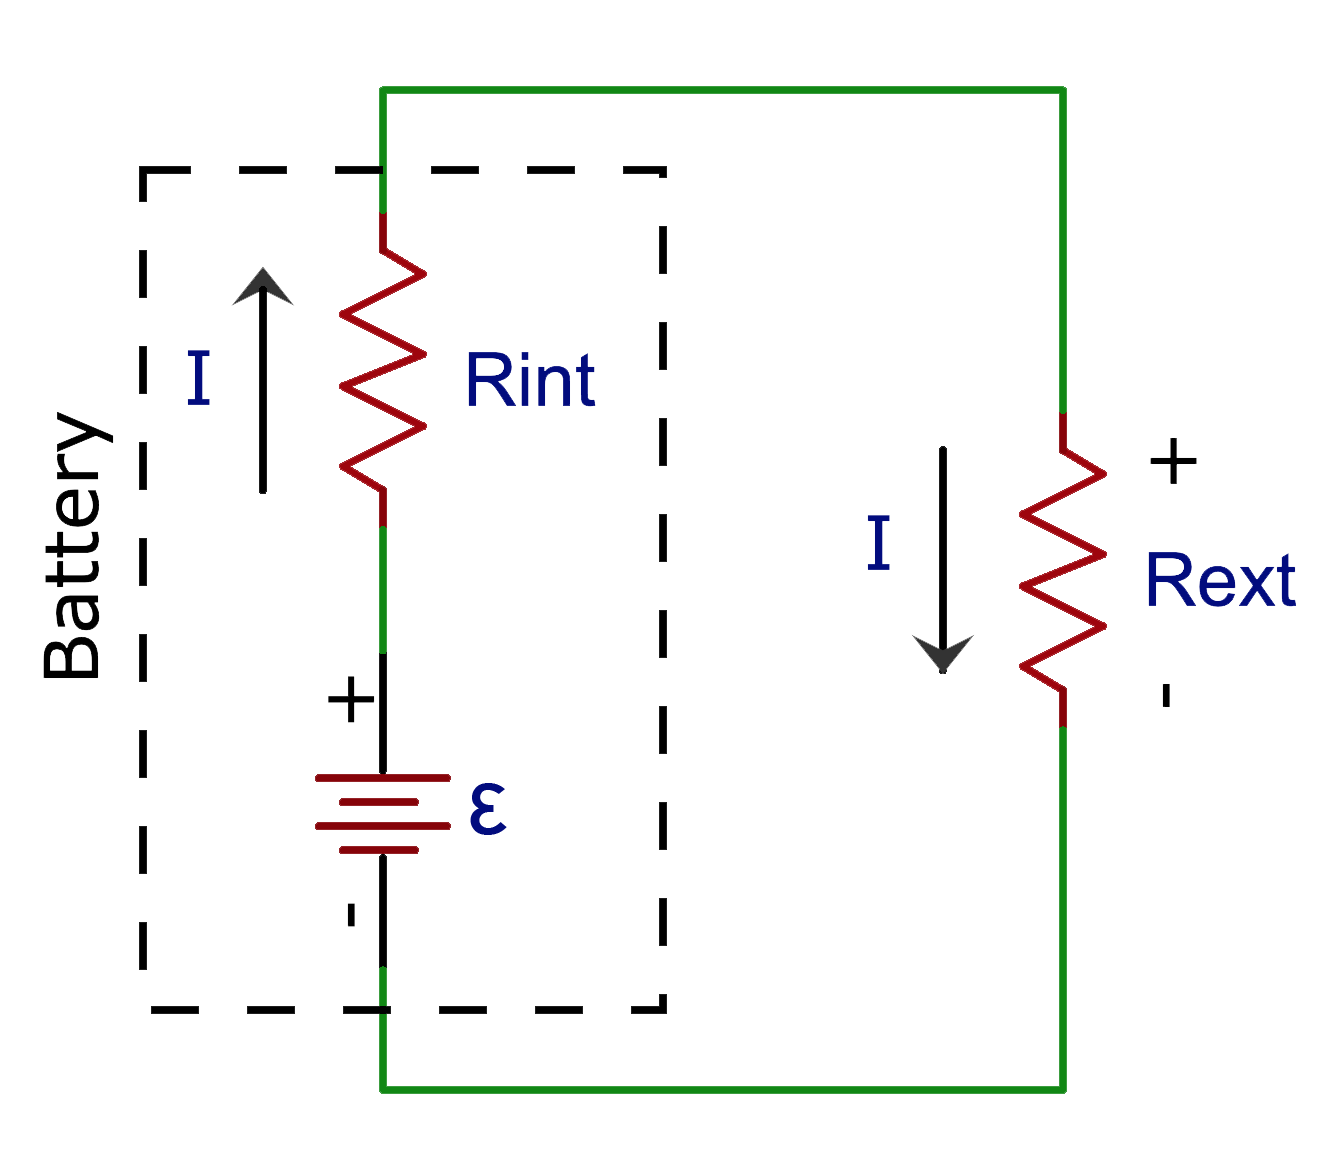
\includegraphics[width=\columnwidth]{images/lab3_1.png}
    \captionof{figure}{Schematic for a simple circuit with a battery and external resistor}
    \label{fig:first}
    \medskip
\endgroup

\noindent Figure \ref{fig:first} above simplifies the internal resistance of the battery system (battery, wires, screw terminal, etc.) to a single equivalent resistor. In principal, the internal resistance was determined by measuring the supplied voltage,  the voltage drop across $R_{ex}$, and manipulating Ohm's law to determine the supplied current. 


\smallskip
\section{Circuit Assembly and Measurements}

\noindent The simple schematic was recreated in CAD as shown in Figure \ref{fig:third}. The simulation illustrates the idea of an internal resistor. Assuming no internal resistance for a battery in an ideal circuit, the voltage across $R_{ex}$ would have been the voltage supplied by the battery.\\

\noindent The circuit above was recreated using a breadboard, as shown in Figure \ref{fig:second}. Internal resistance in the set-up was assumed to be the equivalent resistance of the battery, the wire, and the screw terminal.

\begingroup
    \medskip
    \centering
    %width=\columnwidth
    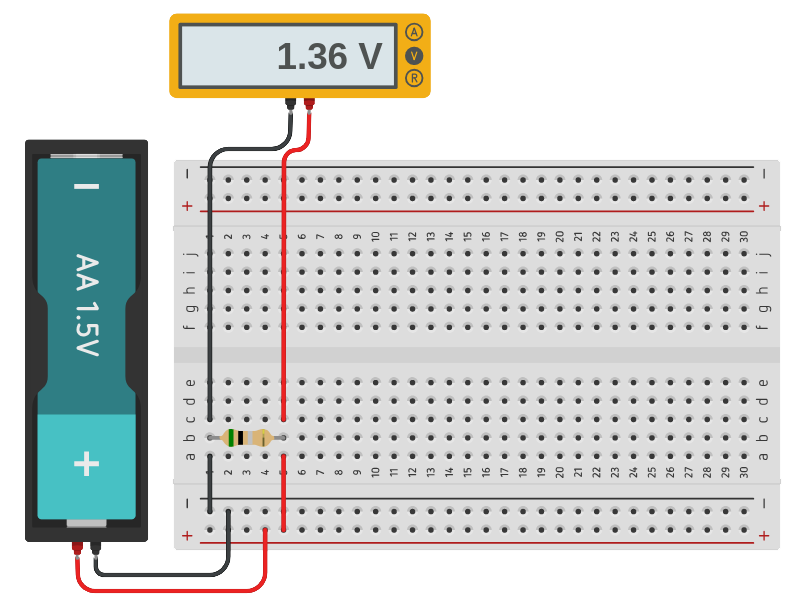
\includegraphics[width=\columnwidth]{images/lab3_2.png}
    \captionof{figure}{CAD layout recreating the Thevenin circuit}
    \label{fig:third}
    \medskip
\endgroup
\\

\noindent A charged battery was snapped into a battery terminal and its cables were screwed into a screw terminal. The screw terminal was positioned on the breadboard to allow for the external resistor to be in series with the battery. Three resistors (5.1 \ohm, 10.0 \ohm, and 15.1 \ohm) were used for two batteries (alkaline and nickel metal-hydride). First, the open circuit voltage ($V_{oc}$ was measured by applying a multimeter's terminals to the ends of the battery terminal. Next, the voltage drop across $R_{ext}$ was measured by applying the multimeter terminals to the screw terminal (Figure \ref{fig:second}).

\begingroup
    \medskip
    \centering
    %width=\columnwidth
    \includegraphics[width=\columnwidth]{images/lab3_3.png}
    \captionof{figure}{A simple Thevenin circuit prototyped on a breadboard}
    \label{fig:second}
    \medskip
\endgroup


\section{Ohm's Law Calculations}

\noindent The resistance value of the internal resistor is important to know as it contributes to the drop in output voltage as well as limits the current coming out of the battery. The resistor value can be calculated by manipulating Ohm's law.\\ 

\noindnet First, Ohm's law was rewritten to calculate the current flowing through the circuit, made possible because the $V_{ext}$ was measured for each $R_{ext}$ value. Equation \ref{eq:currentcalc} shows the current calculated using a $5.1 \ohm$ resistor and a nickel metal hydride battery (see Figure \ref{fig:fifth}).

\begin{equation}
I = \frac{V_{ext}}{R_{ext}} = \frac{1.300V}{5.1\ohm} = 0.255A
\label{eq:currentcalc}
\end{equation}

\noindent Having obtained the current in the circuit, the voltage drop across $R_{int}$ was calculated by finding the difference between $V_{oc}$ and $V_{ext}$. Ohm's law was once again used to find $R_{int}$ as follows:

\begin{equation}
R_{int} = \frac{V_{oc}-V_{ext}}{I} = \frac{1.376V-1.300V}{0.255A} = 0.298\ohm
\label{eq:rintcalc}
\end{equation}

\noindent Figure \ref{fig:fifth} and figure \ref{fig:sixth} show the calculated results for all 6 trials encompassing the three resistor values and two battery types. 

\begingroup
    \medskip
    \centering
    \def\arraystretch{1.5}
    \begin{tabular}{lccc}
    \toprule
    \textbf{Trial \#} & 1 & 2 & 3 \\
    \toprule
    \textbf{V$_{oc}$ (V)} & 1.376 & 1.375 & 1.374 \\
    \hline
    \textbf{R$_{ext}$ (\ohm)} & 5.1 & 10.0 & 15.1 \\
    \hline
    \textbf{V$_{ext}$ (V)} & 1.300 & 1.331 & 1.347 \\
    \hline
    \textbf{I (A)} & 0.255 & 0.133 & 0.089 \\
    \hline
    \textbf{R$_{int}$ (\ohm)} & 0.298 & 0.331 & 0.303 \\
    \hline
    \textbf{P$_{int}$ (W)} & 0.019 & 0.006 & 0.002 \\
    \hline
    \textbf{P$_{Total}$ (W)} & 0.351 & 0.183 & 0.123 \\
    \hline
    \textbf{P$_{\% \: lost\: in\: battery}$ (\ohm)} & 5.523 & 3.200 & 1.965 \\
    \hline
    \textbf{Average R$_{int}$ (\ohm)} &\multicolumn{3}{c}{0.310} \\
    \hline
    \textbf{Average V$_{oc}$ (V)} &\multicolumn{3}{c}{1.375} \\
    \toprule
    \end{tabular}
    \captionof{figure}{Various data points obtained and calculated for Nickel metal-hydride battery}
    \label{fig:fifth}
    \medskip
\endgroup


\begingroup
    \medskip
    \centering
    \def\arraystretch{1.5}
    \begin{tabular}{lccc}
    \toprule
    \textbf{Trial \#} & 1 & 2 & 3 \\
    \toprule
    \textbf{V$_{oc}$ (V)} & 1.615 & 1.614 & 1.625 \\
    \hline
    \textbf{R$_{ext}$ (\ohm)} & 5.1 & 10.0 & 15.1 \\
    \hline
    \textbf{V$_{ext}$ (V)} & 1.477 & 1.540 & 1.570 \\
    \hline
    \textbf{I (A)} & 0.290 & 0.154 & 0.104 \\
    \hline
    \textbf{R$_{int}$ (\ohm)} & 0.477 & 0.481 & 0.529 \\
    \hline
    \textbf{P$_{int}$ (W)} & 0.040 & 0.011 & 0.006 \\
    \hline
    \textbf{P$_{Total}$ (W)} & 0.468 & 0.249 & 0.169 \\
    \hline
    \textbf{P$_{\% \: lost\: in\: battery}$ (\ohm)} & 8.545 & 4.585 & 3.385 \\
    \hline
    \textbf{Average R$_{int}$ (\ohm)} &\multicolumn{3}{c}{0.495} \\
    \hline
    \textbf{Average V$_{oc}$ (V)} &\multicolumn{3}{c}{1.618} \\
    \toprule
    \end{tabular}
    \captionof{figure}{Various data points obtained and calculated for Alkaline battery}
    \label{fig:sixth}
    \medskip
\endgroup

\section{Analysis and Discussion}\\

\noindent For the nickel metal hydride battery, it was observed that as $R_{ext}$ increased, the power consumption of $R_{int}$ decreased. This is because increasing the load resistor decreases the current flowing through the circuit, causing the power dissipated in the battery to decrease with the following relation:

\begin{equation}
P = I^{2}R_{int} = (\frac{V_{ext}}{R_{ext}})^2(R_{int})
\label{eq:powercalc}
\end{equation}

\noindent As the relation is exponential, it is expected that increasing the load resistor will lead to an exponential decay of power dissipation. Figure \ref{fig:eighth} confirms this relation, as it depicts the percent power dissipated in the battery exponentially decrease as $R_{ext}$ increases. On the other hand, while the absolute power dissipated by the external resistor decreases (see Figure \ref{fig:fifth} and Figure \ref{fig:sixth}), the percentage power dissipated in fact increases for the external resistor and this relation is depicted in Figure \ref{fig:ninth}.\\

\noindent In summary, the power dissipated across both internal and external resistors decreases as the external resistor value is increased. However, the external resistor absorbs a higher percentage of the power. Thus, the rate at which the power dissipation in watts drops for the $R_{int}$ is greater than that of $R_{ext}$.

\begingroup
    \medskip
    \centering
    %width=\columnwidth
    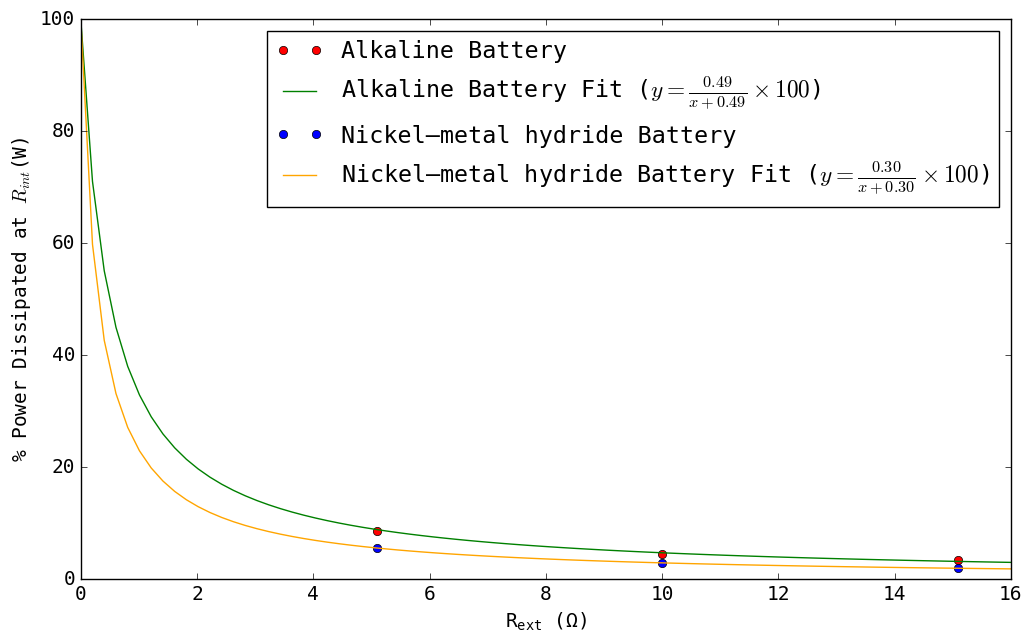
\includegraphics[width = \columnwidth]{images/lab3_graph1_1.png}
    \captionof{figure}{Percent power dissipated by the internal resistor against the external resistor}
    \label{fig:eighth}
\endgroup

\begingroup
    \medskip
    \centering
    %width=\columnwidth
    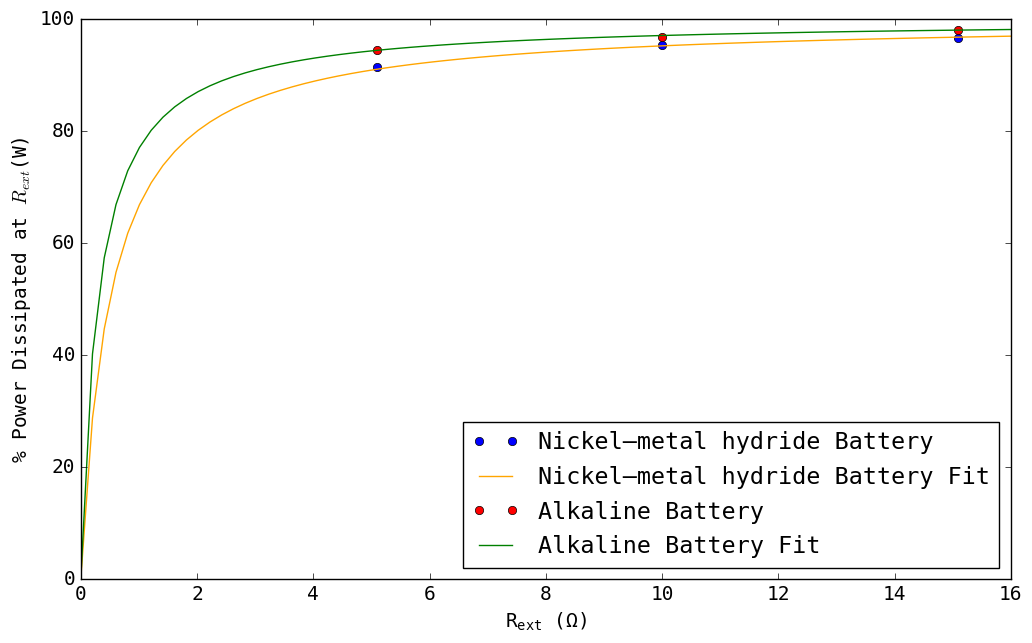
\includegraphics[width = \columnwidth]{images/lab3_graph1_2.png}
    \captionof{figure}{Percent power dissipated by the external resistor against the external resistor}
    \label{fig:ninth}
    \medskip
\endgroup


\noindent Another relation can be made between current, $I$, and $V_{ext}$. Ohm's law says that the relationship between current and voltage is linear, which is confirmed by Figure \ref{fig:seventh}. Dividing any given current by its corresponding voltage drop provides the resistor value $R_{ext}$.

\begingroup
    \medskip
    \centering
    %width=\columnwidth
    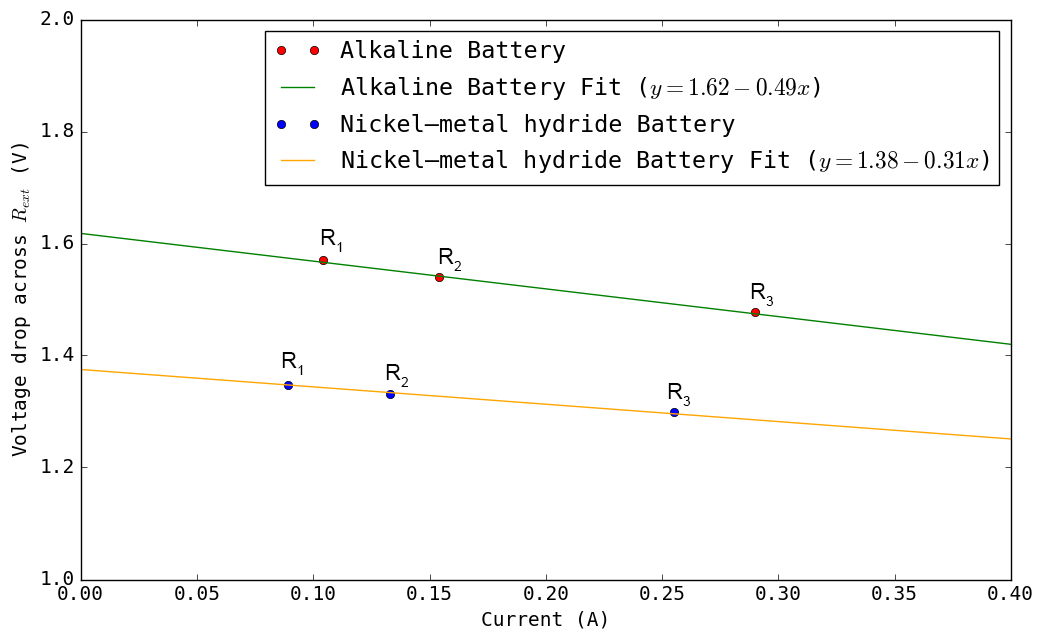
\includegraphics[width =\columnwidth]{images/lab3_graph2.jpg}
    \captionof{figure}{Current graphed against the voltage drop across the exterior resistor}
    \label{fig:seventh}
    \medskip
\endgroup

\noindent Interestingly, looking at the equation of the line of best fit in Figure \ref{fig:seventh}, it was observed that the slope is equivalent to that of the internal resistance of the circuit. This relation can be explained by the following derivations: 

\begin{equation}
V_{oc} = I (R_{int} + R_{ext}) 
\label{eq:currentcalc}
\end{equation}

\begin{equation}
V_{oc} = I R_{int} + I  R_{ext}
\label{eq:currentcalc}
\end{equation}

\begin{equation}
V_{oc} = I R_{int} + V_{ext}
\label{eq:currentcalc}
\end{equation}

\begin{equation}
R_{int} = \frac{V_{oc} - V_{ext}}{I}
\label{eq:currentcalc}
\end{equation}

\begin{equation}
V_{ext} = V_{oc} - I(R_{int})
\label{eq:currentcalc}
\end{equation}


\noindent More obviously, the y-intercept is equivalent to the $V_{oc}$ of the circuit, which is by definition when the current in the circuit goes to zero. 

\section{Discussion and Conclusion}\\

\noindent Internal resistance of two different kinds of batteries (Nickel metal-hydride and Alkaline) were calculated. 3 different external loads (5 \ohm, 10 \ohm, 15 \ohm) were used to take the measurements. The voltage drop across the resistors and the open circuit voltage of the battery was used to carryout calculations. Metal-hydride battery was found to have $0.31 \ohm$ and Alkaline was found to have $0.495 \ohm$ of internal resistance. Finally, the collected data was fit into a curve and the power dissipated at the internal resistor and external load was compared. This data can be useful for determining the efficiency of the batteries and better estimating their lifetime. Understanding the internal resistance aids in indicating the battery performance. Furthermore, as the battery heats up, the resistance increases; therefore, internal resistance may also be an indicator of battery temperature.

%\appendices
%\section{Proof of the First Zonklar Equation}
%Appendix one text goes here.

%\section*{Acknowledgment}

\printbibliography

\end{document}